\chapter{Introduction}
This documentation contains information about the specifications, design, architecture and functionality of the dynamometer named Rolling Road. The system is designed with the goal of testing the performance of the electrically propulsed car 'AU2'.

It should be noted that the system is designed to work with 'AU2' and 'Rolling Road GUI'. These are treated as separate systems and it is recommended that the reader reads each documentation, in order to get a complete overview of the systems.

\begin{figure}[H]
	\centering
	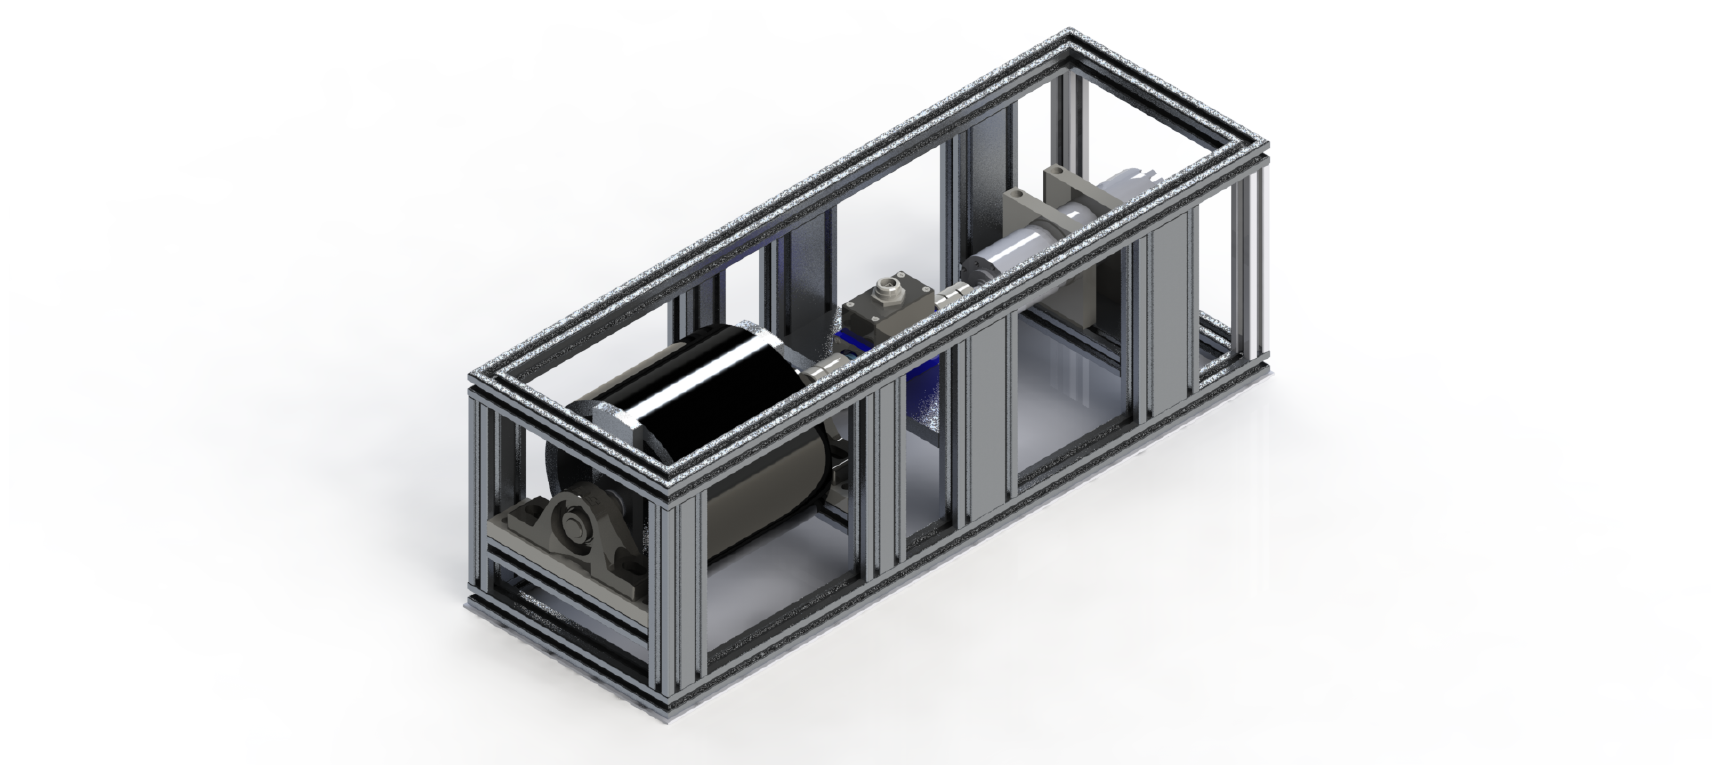
\includegraphics[width=0.5\linewidth]{Introduction/Model}
	\caption{Computer generated model of the system}
	\label{fig:System_model}
\end{figure}

\section{Preface}
Rolling Road is actually an improved build of a previous system dubbed 'Teststand til Børsteløs
DC-Motor'\cite{BAC_rullefelt}. Many of the calculations and tests will reappear in this documentation and in some cases they will be omitted completely and the previous documentation will simply be referenced instead. 

The previous system was designed to test an electric car dubbed Zenith33\cite{BAC_zenith33}, which can be viewed as a precursor to AU2. Both AU2 and Zenith33 utilizes the same DC-motor but differ in internal components and external structure. As AU2 was being developed in parallel with Rolling Road (and was not complete during the writing of this documentation), most of the tests and calculations in this documentations are done using the Zenith33. During the writing of this documentation it is assumed that AU2 and Zenith33 is the same car and wille simply be refered to as AU2.

\newpage
\section{System description}
The primary purpose of the system is to measure the performance of an electrically propulsed car. The system has been designed with 'AU2' in mind, but can also be used to test individual motors; as long as they meet the specifications.

The performance is tested in order to optimize the propulsion-algorithm in the car's motor controller. Testing is done by placing the car on top of the dynamometer and connecting the car's battery to the measurement-system. The performance is measured as the amount of electrical power from the battery which is directly converted to the mechanical energy which spins the car's wheel.

During the test the system will collect data from the test-drive and send it to the 'Rolling Road GUI' where the data will be displayed graphically. The user is also able to regulate the amount of torque required to spin the roll in the dynamometer, by using this GUI, which makes it possible to simulate an elevation. 

A quick overview of the system is shown in \ref{fig:System_overview}. Neither the GUI nor 'AU2' are part of this system, but should be connected for complete functionality.

\begin{figure}[H]
	\centering
	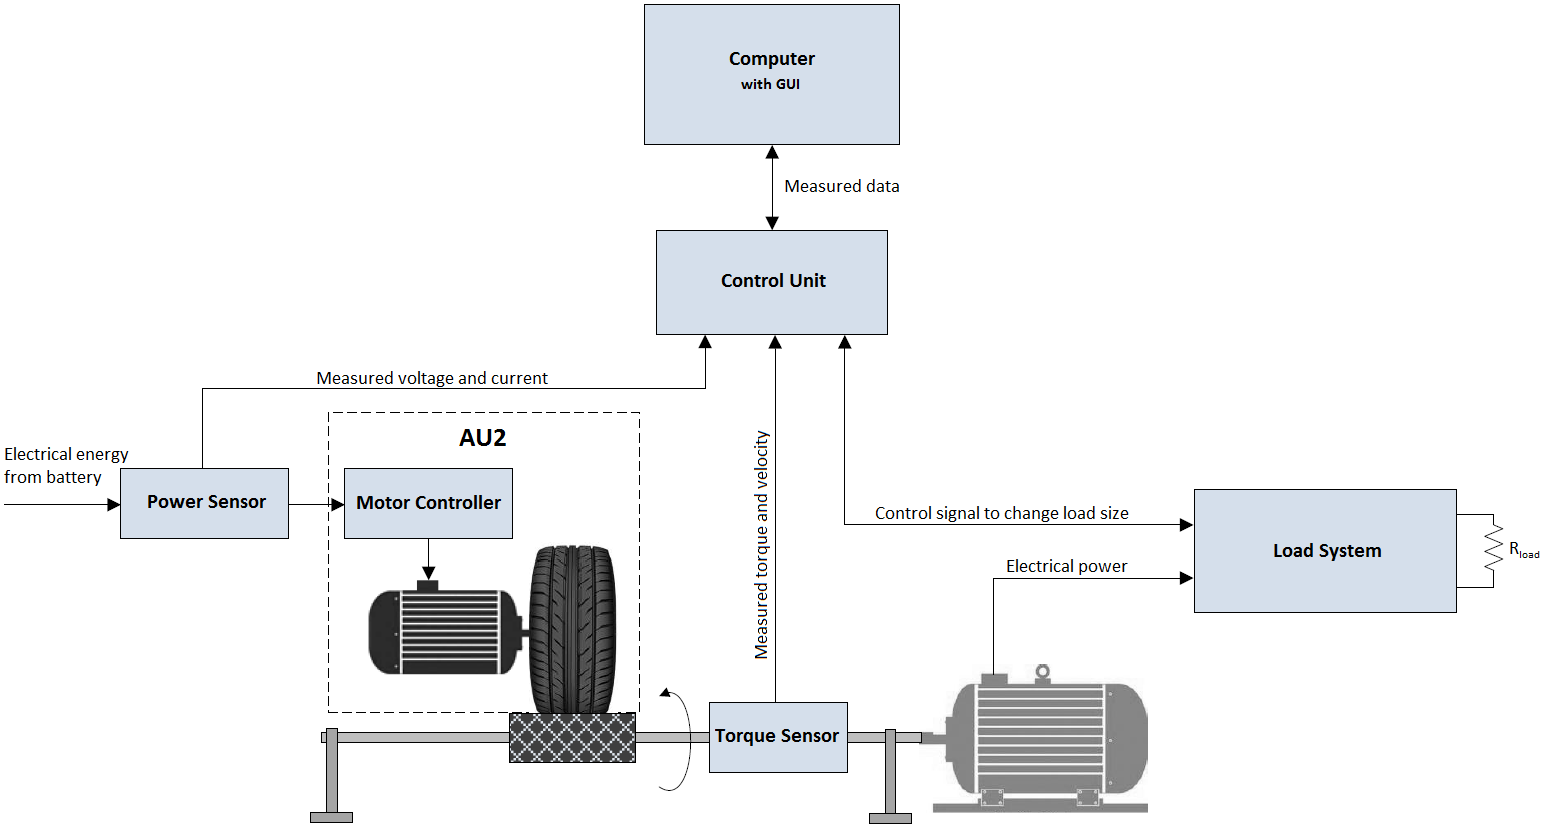
\includegraphics[width=1\linewidth]{Introduction/Overview}
	\caption{System overview}
	\label{fig:System_overview}
\end{figure}

\newpage
\section{List of terms}
The following list explains the various terms which has been used to refer to certain parts or subsystems.
\begin{itemize}
	\item \textbf{AU2}\\
	Refers to the car which is being developed simultaneously as the dynamometer in order to optimize the car's performance.
	\item \textbf{SEM}\\
	Refers to the Shell Eco-Marathon which AU2 is designed to compete in.
	\item \textbf{GUI}\\
	Refers to the Rolling Road GUI which must loaded on a PC which is connected to Rolling Road, in order to get a visual representation of the measured data.
	\item \textbf{Load System}\\
	Refers to the system which must dissapate the generated power from the Rolling Road DC-generator. This is done through an electrical resistive load.
	\item \textbf{PSoC}\\
	Refers to the CY8CKIT-059 PSoC 5LP Prototype Kit which is used as the Control Unit in the system.
	\item \textbf{Control-box}\\
	Refers to the electrical enclosure which contains the electrical systems - excluding the passive parts of the Load System. 
	\item \textbf{Load-plate}\\
	Refers the plate where the passive parts of the Load System (power resistors and super capacitor) are placed. These components are placed externaly due to their size and the generated heat.
	\item \textbf{Subject}\\
	Can be either AU2 or simply a stand-alone test-motor.
	\item \textbf{Previous Dynamometer}\\
	Refers to the previous system which was discussed in the Preface. This system was dubbed Teststand til Børsteløs DC-Motor' and was developed by Seyyid Öztoprak and Simon L. Madsen.
\end{itemize}